% !TEX root = main.tex

\section{Analysis}

The following analysis will be presented in two parts, one which will be before filtering with timedomain response of the two signals and then the frequency analysis of these with poles and zeroes. Next an appropriate filter will be applied and the two signals will again be analysed as previously explained.

\subsection{Before filtering}

\subsubsection{Timedomain analysis}

Firstly an formal analysis of the man and the womans voice saying "Hej Lasse" in the timedomain. In \cref{fig:time_man} the signal for the man can be seen, with the time in seconds on the x-axis and the magnitude on the y-axis and similarily the womans signal is shown in \cref{fig:time_woman}.

\begin{figure}
\centering
\begin{subfigure}{0.45\textwidth}
	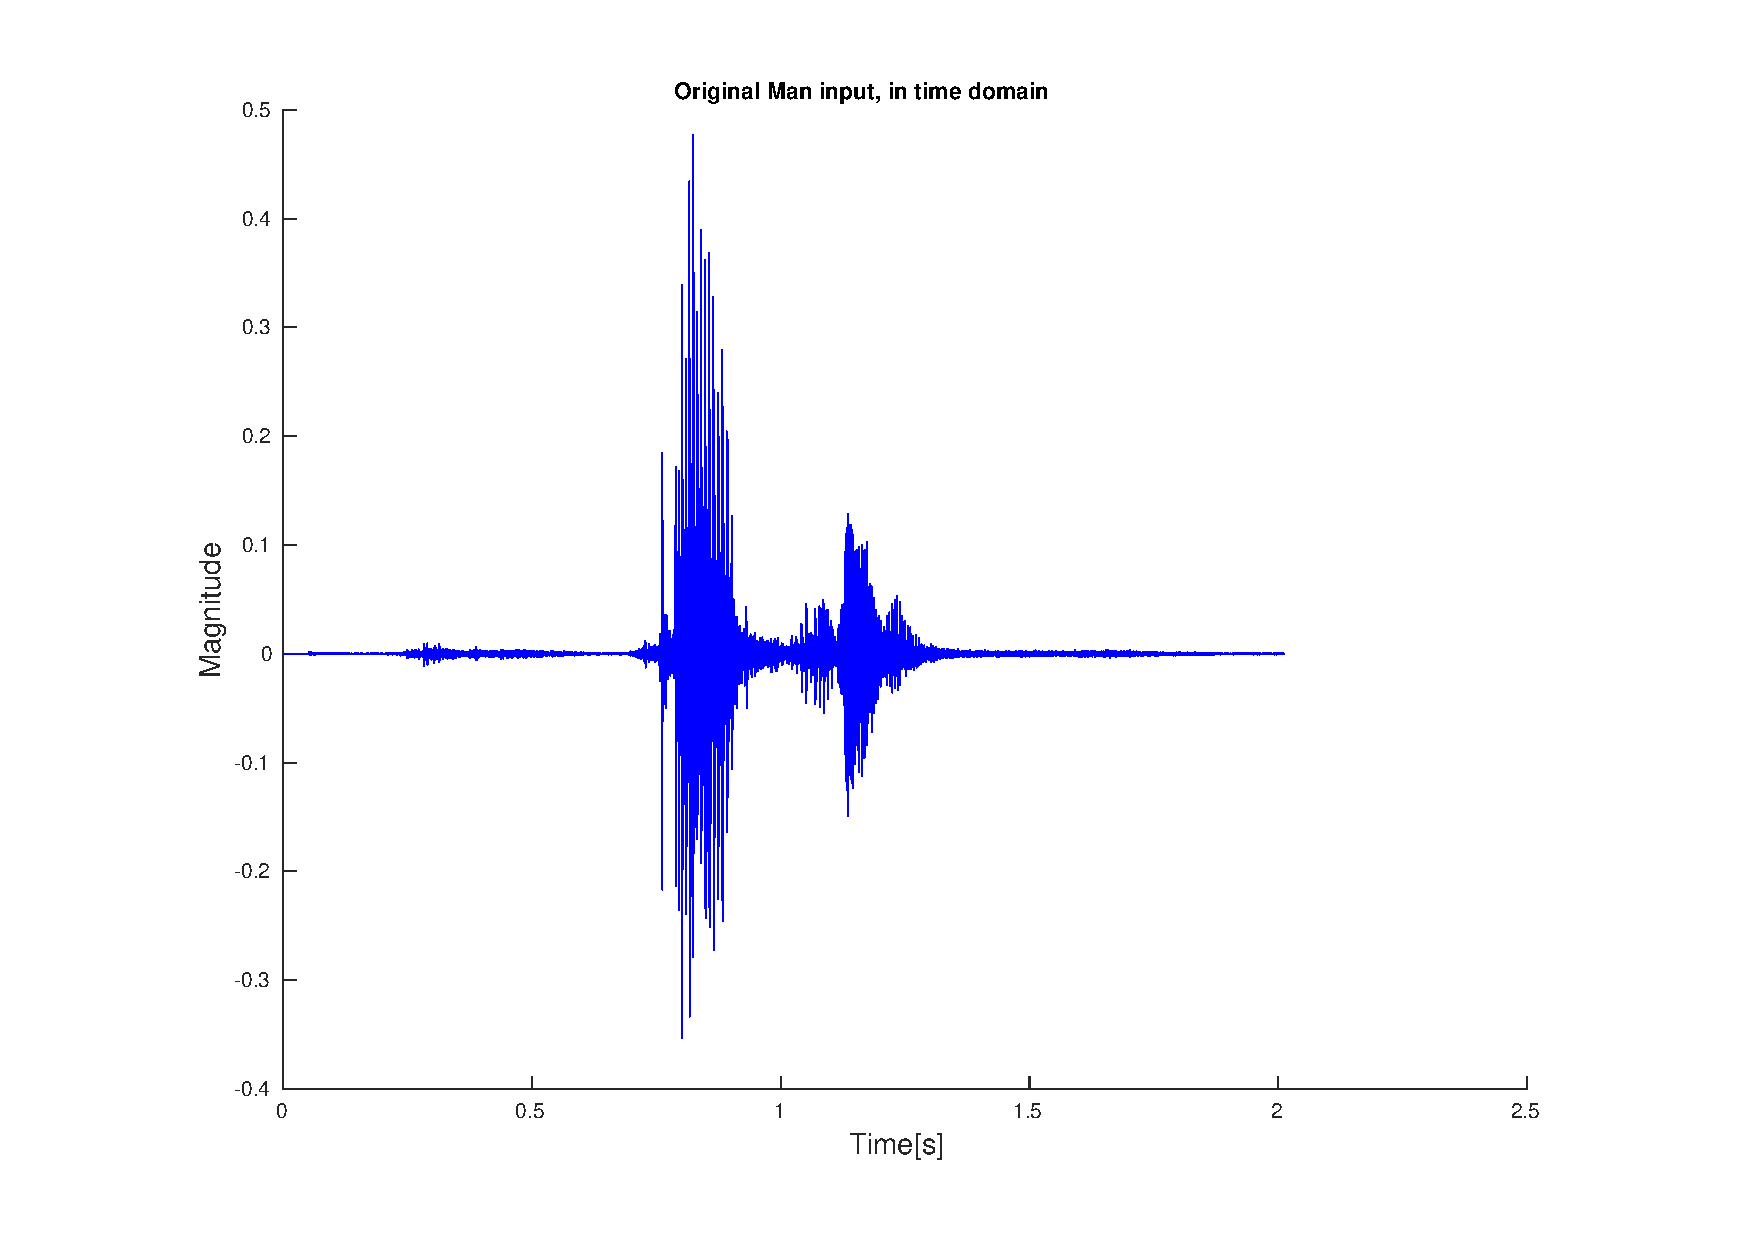
\includegraphics[width=\textwidth]{OrgTid_Man.pdf}
	\caption{The time domain signal of the man}
	\label{fig:time_man}
\end{subfigure}
\quad
\begin{subfigure}{0.45\textwidth}
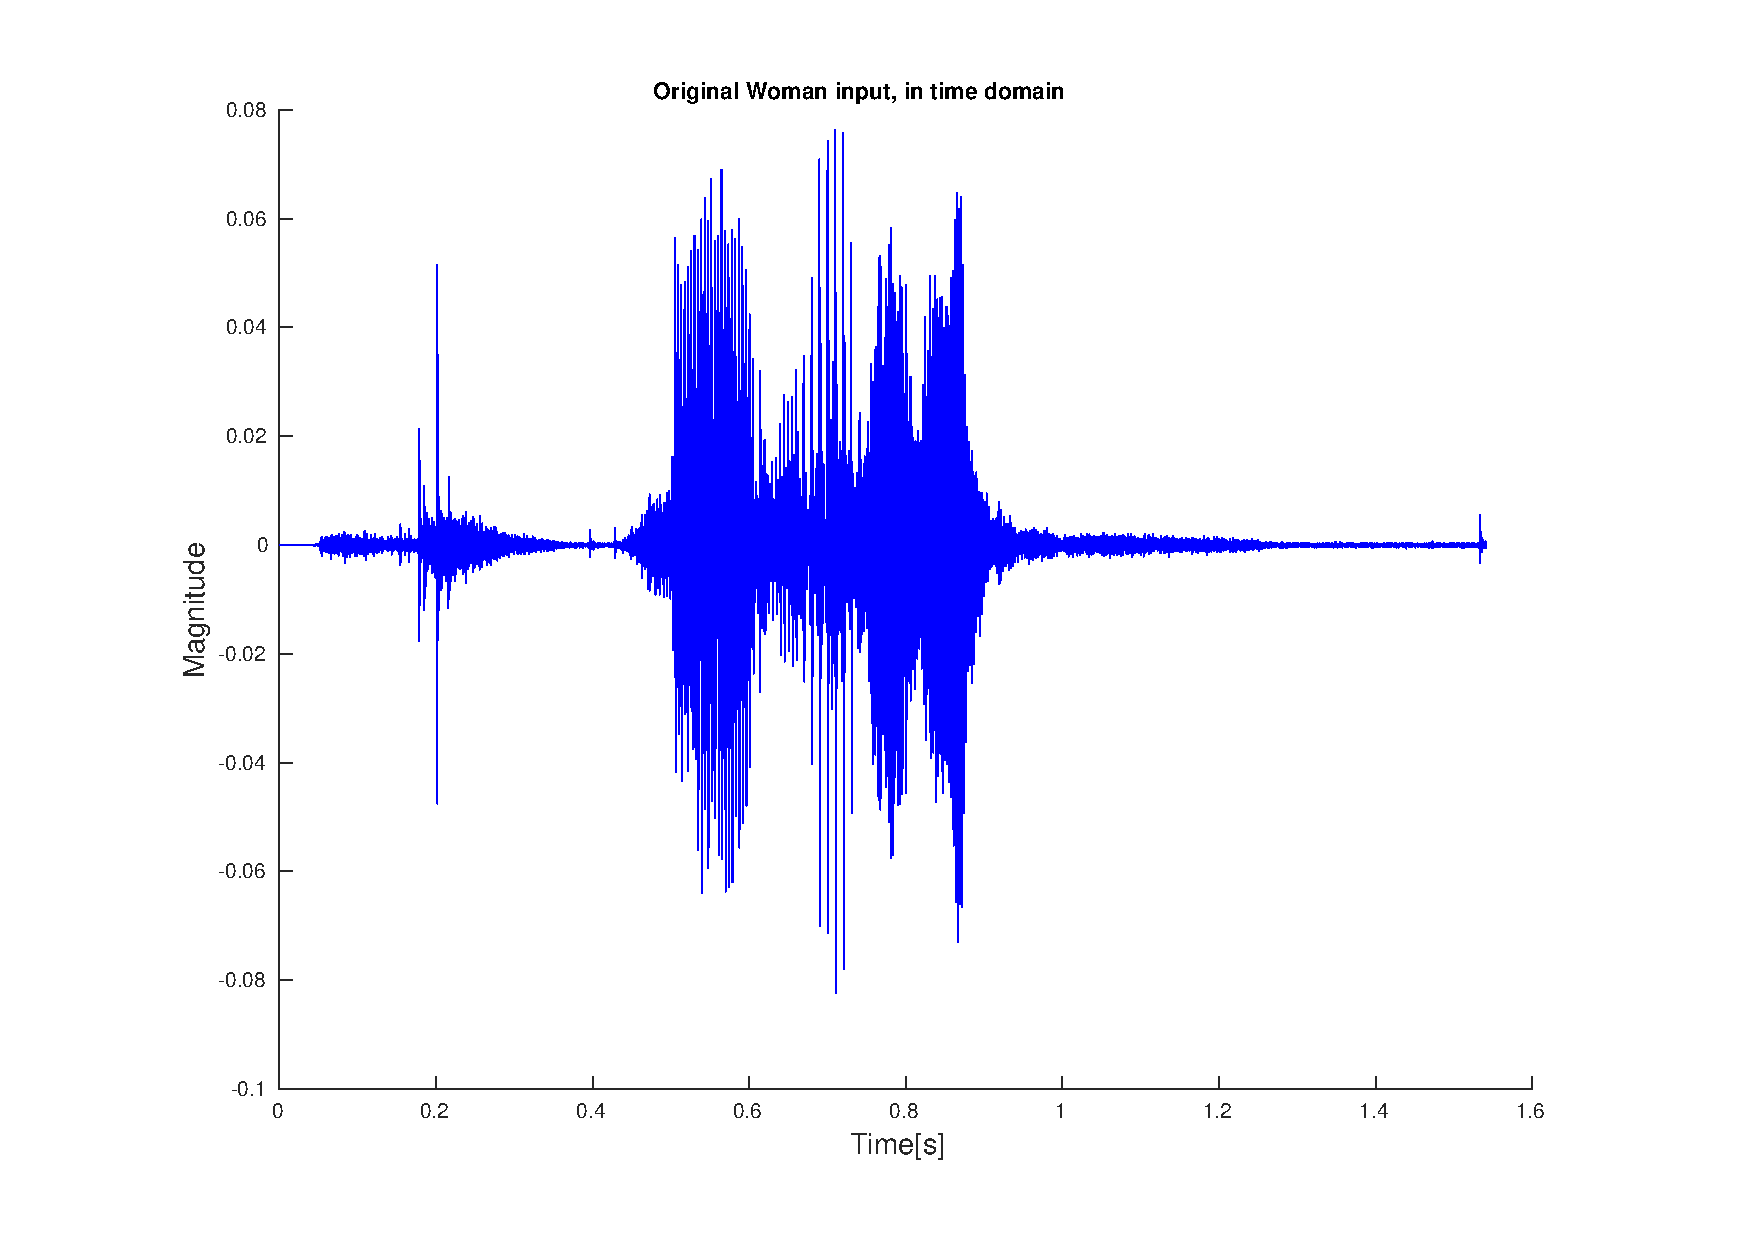
\includegraphics[width=\textwidth]{OrgTid_Woman.pdf}
\caption{The time domain signal of the woman}
\label{fig:time_woman}
\end{subfigure}
\caption{The timesamples of a man and a woman saying "Hej Lasse"}
\label{fig:time_WoMan}
\end{figure}

\subsubsection{Fourier transform with FFT}

The fourier transform will show the characteristics of the male and female voice. In \cref{fig:WoManFFT} the fourier transform based of the two privious signals seen in \cref{fig:time_WoMan} - in red the male signal and in blue the female signal.

\begin{figure}[bh]
\centering
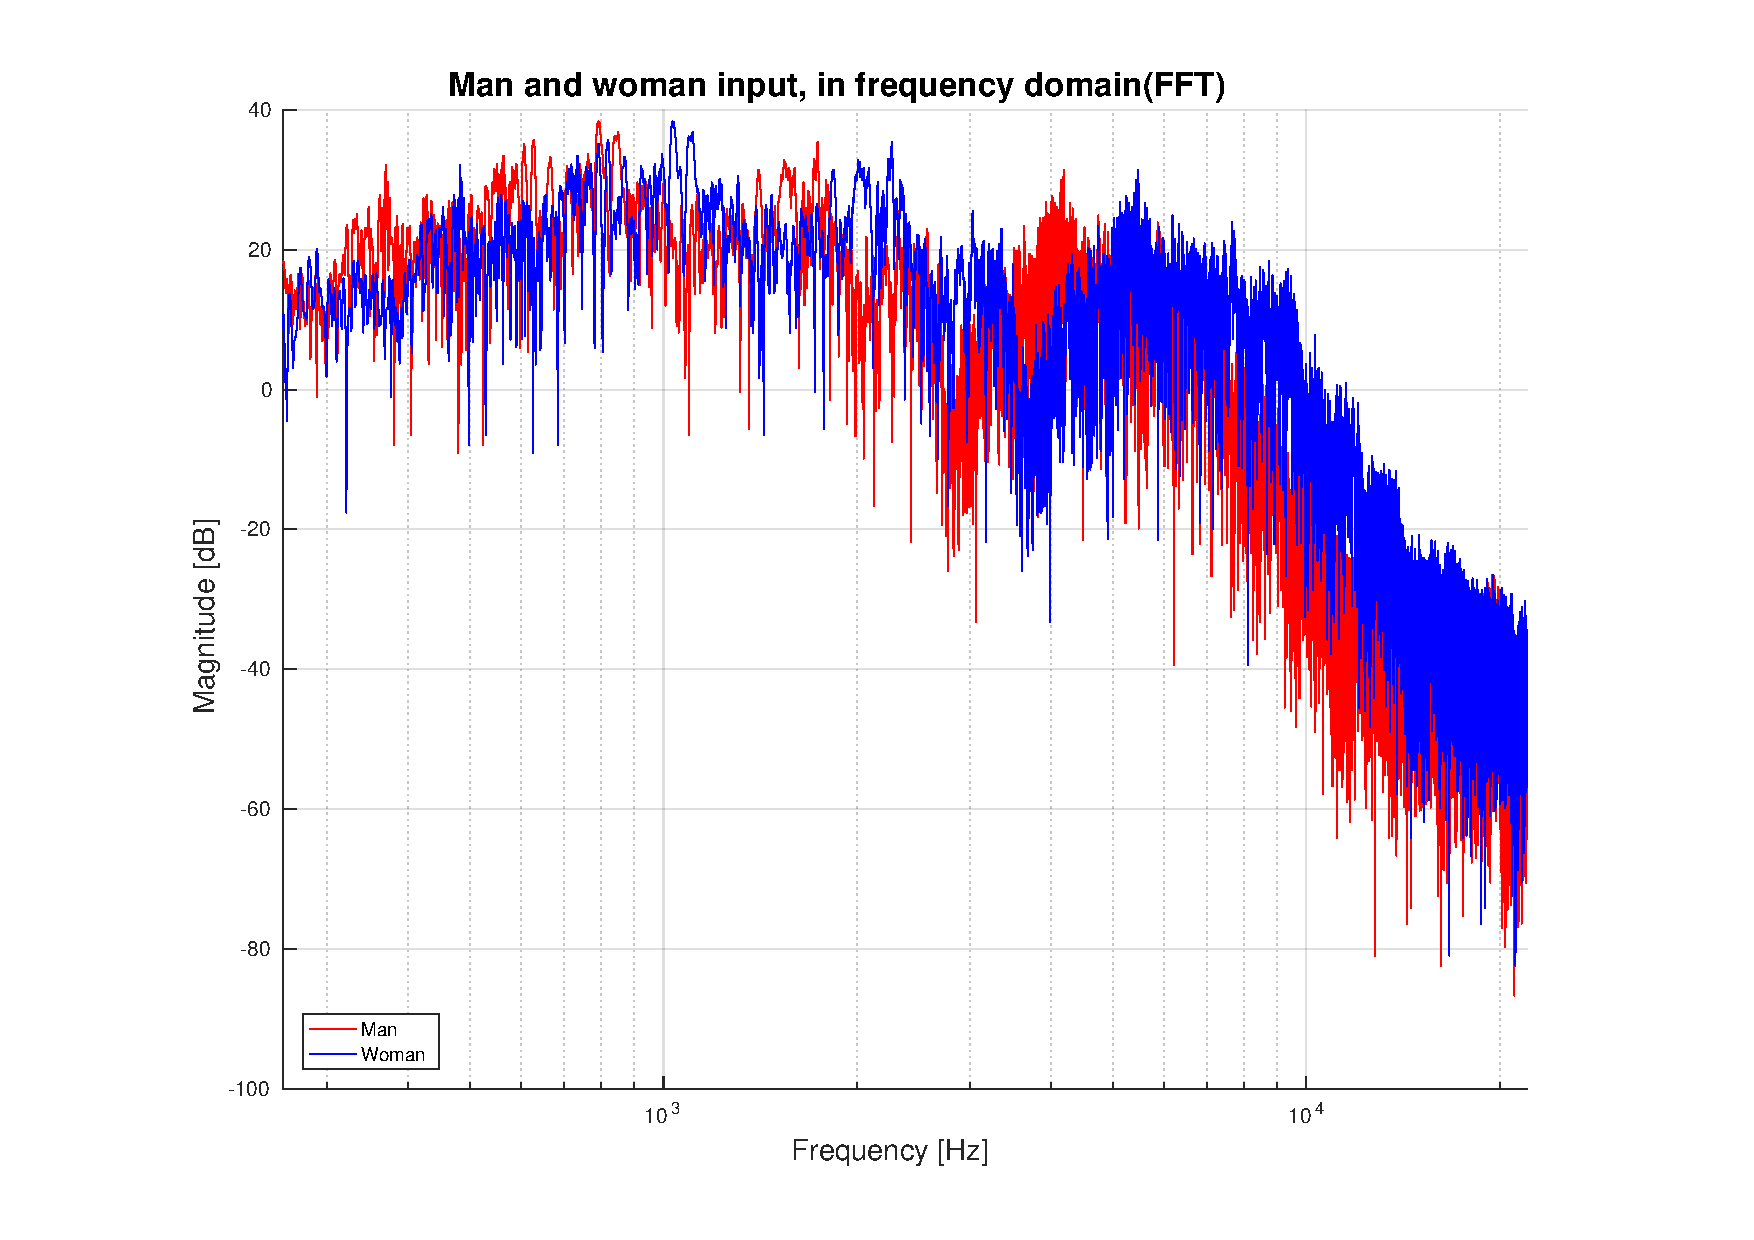
\includegraphics[width=\textwidth]{OrgFreq_WoMan.pdf}
\caption{The frequency analysis of the man and woman}
\label{fig:WoManFFT}
\end{figure}

\subsubsection{Phaseshift}

%Insert about phaseshift

\subsection{Filtering}

\subsubsection{Highpass filter}
Next up is filtering the signal, which will be done with an highpass filter. From \cref{fig:WoManFFT} an cutoff estimation of \SI{3500}{\hertz} for the female voice and \SI{2800}{\hertz} for the male voice. These two cutoff frequencies will be switch for the two signals to see which effect this will bring our signal.

The highpassfilter is implemented as a function in matlab and can be seen in the following code example:

\begin{minted}{matlab}
function [figfreq, figHz] = HP(cutFreq, Fs, y, figOrgFreq, figfreqz)
N = length(y);
frequency_samples = [0:Fs/N:(Fs-(Fs/N))];
HighPass = cutFreq/(Fs/2);
HiPass = fir1(70,HighPass,'high');
figfreq = figure(figfreqz);
hold off
title('Filter characteristics');
hold on
freqz(HiPass,1);

% save and visualise 
tic
yHP = filter(HiPass,1,y);
toc
name = ['HP_', num2str(cutFreq), '_Hz.flac'];
audiowrite(name, yHP, Fs);
YHP = fft(yHP);
YdBHP = 20*log10(abs(YHP));

% Plot of discrete fourier transform
figHz = figure(figOrgFreq);
hold off
title(['Original and HP(512 Hz)', ' in frequency domain(FFT)']);
hold on
semilogx(frequency_samples(1:N/2), YdBHP(1:N/2), 'b');
legend({'original', 'highpass'}, 'FontSize', 16);
legend('Location','best');
end
\end{minted}


Notice that the filtered signal i stored as a .flac file, which also will be displayed. The filtered signal can be seen in \cref{fig:HPMAle} for the male and female in \cref{fig:HPFemale}. The filtered signals are somewhat disapointing to listen to, because it simply sounds like 

\begin{figure}
\centering
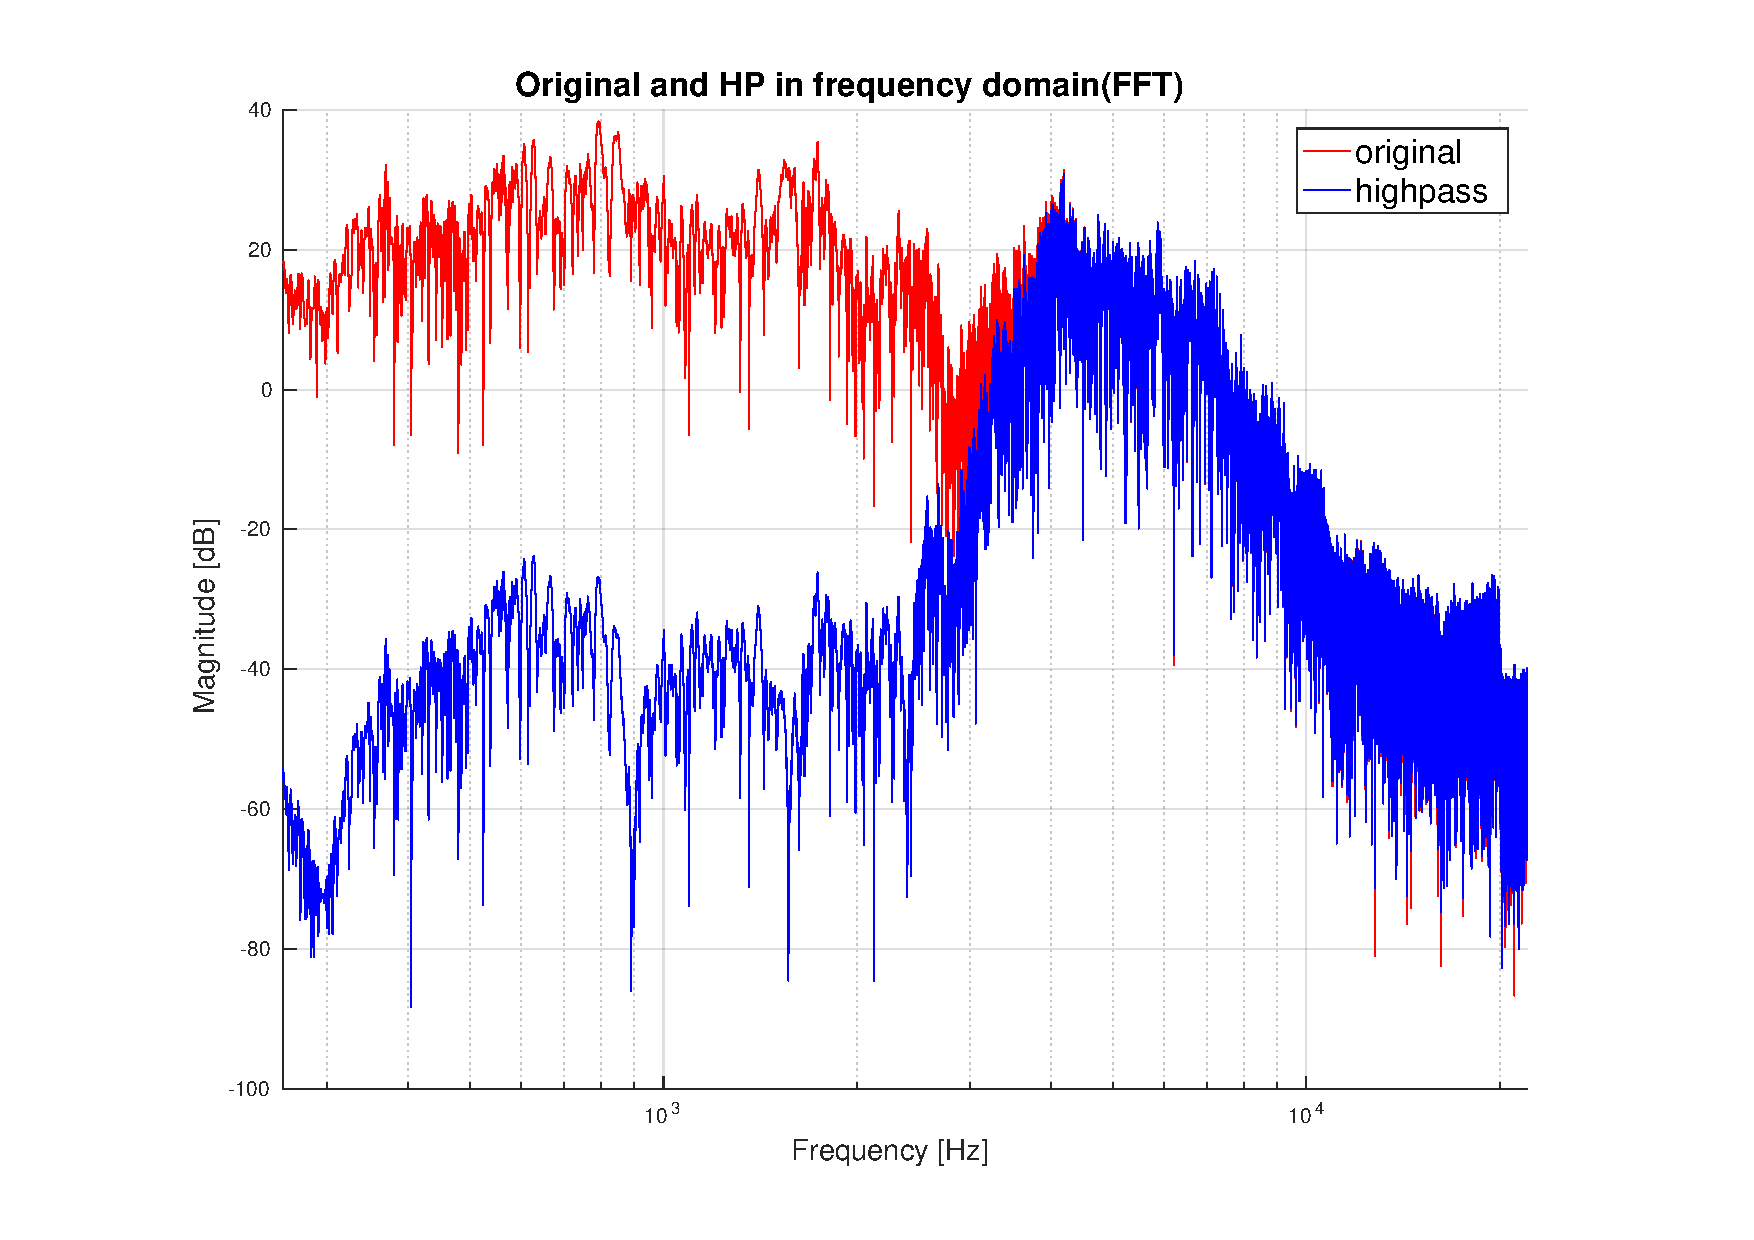
\includegraphics[width=\textwidth]{HPnormFreq_Man.pdf}
\caption{The highpass filtered signal of the male input}
\label{fig:HPMAle}
\end{figure}

\begin{figure}
	\centering
	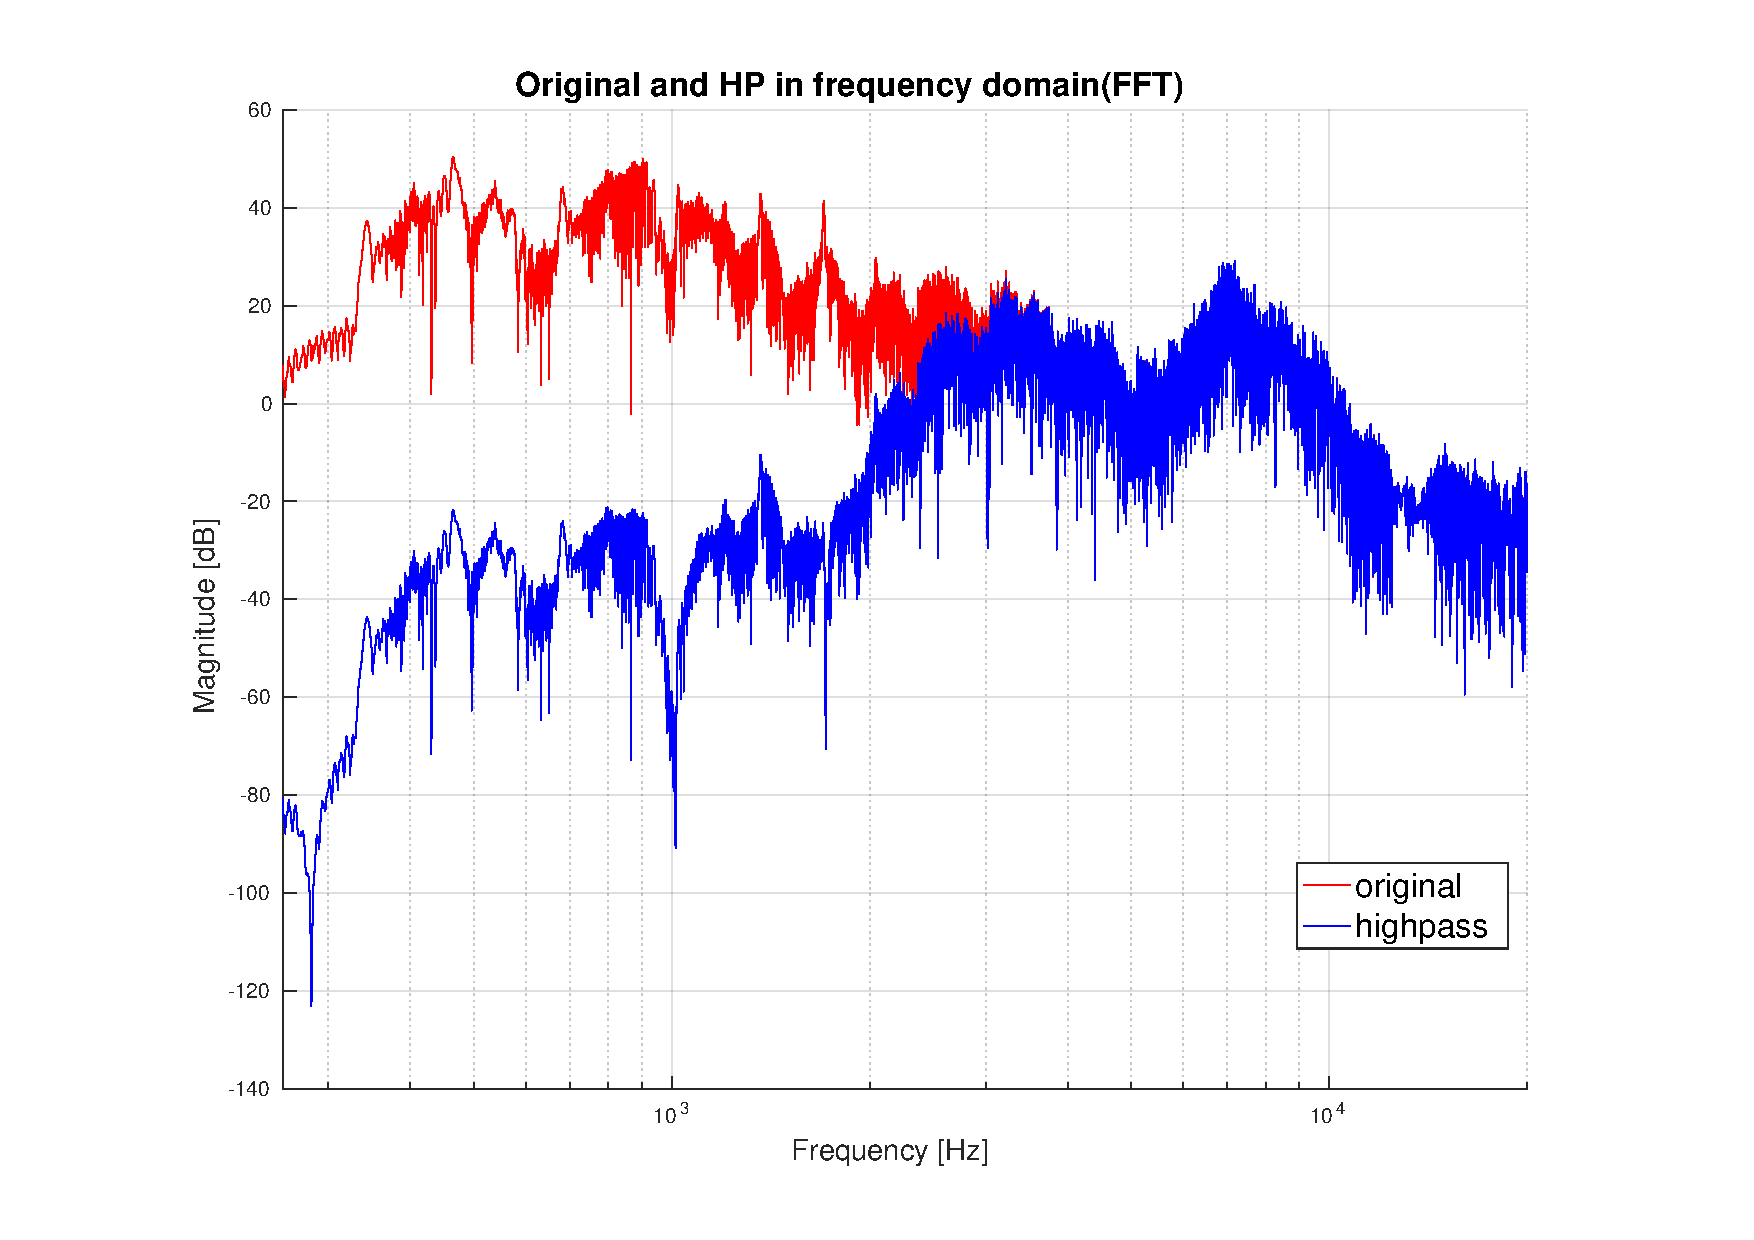
\includegraphics[width=\textwidth]{HPnormFreq_Woman.pdf}
	\caption{The highpass filtered signal of the female input}
	\label{fig:HPFemale}
\end{figure}

% Insert picture of highpass filtering male and female

% Insert code of function

%\subsubsection{Bandstop filter} --- Is this needed?

\subsubsection{Fourier transform with FFT}
The signal will once again be fourier transformed after the filtering. 

% Insert fig


\subsubsection{Phaseshift}

%Insert about phaseshift